\chapter{Double-sided VXD: PLUME}
\label{chap:vxd}

%  The signature of physics interest is essentially done by heavy flavour study.
%  To study the Higgs boson and to understand more precisely the nature of this boson, its coupling with the other \gls{SM} particles is important.
%  The capacity of identifying and being able to reconstruct the decay of t, b, c quarks and $\tau$ leptons is mandatory for a future high energy physics experiment.
%  Contrary to the \gls{LHC}, the vertex detector at the \gls{ILC} should be able to distinguish the c quark from the b quark.
%  This chapter deals with the requirements for a vertex tracker able to extrapolate particle tracks back to their production.
%  Firstly, the main parameters that lead the building of a vertex detector are introduced. 
%  Then, the different options for the \gls{ILD} are shown to focus on the double-sided options developed by the \gls{PLUME} collaboration.
%  To finish, the principle of \gls{CMOS} sensors and their use in physics are described.

  The aim of the \gls{ILC} is to perform precise measurement of new and already known particles. 
  It can be achieved only by a proper detector design, driven by flagship measurements like the Higgs coupling to quarks and bosons.
  In fact, the complex events generated at the \gls{LHC} hide the possibility of a direct measurement of the Higgs.
  The vertex detector at the \gls{ILC} should be able to perform an efficient B-meson tagging and to separate $b$ and $c$ quarks.
  The measurement of heavy quark jets and their decay vertices will play a crucial role in the \gls{ILC} physics.
  Along this chapter, the role of the vertex detector and the physics requirements to build one suited for the \gls{ILC} will be presented.
  Then, the different options for the \gls{ILD} are shown to focus on the double-sided options developed by the PLUME collaboration.
  To finish, the principle of \gls{CMOS} sensors and their use in physics are described.

  Since the 1970's, the development of position sensitive silicon radiation sensors has permit to confirm the prediction of the \gls{SM} with a high precision, as well as the discovery of the $t$ quarks.
  To perform precise measurement at the \gls{ILC} to discover new particles or to characterise more accurately new ones, the \gls{VXD} has to be built with respect some flagship measurements.
  For example, to study the coupling of the Higgs with the quarks and bosons, this detector has to be able to separate efficiently the $b$ quarks to the $c$ quarks.

  At the \gls{ILC} flagship measurements such as the Higgs coupling to the quarks and bosons are driving the development of the vertex detector.
  For example, to separate $b$ (1.3 10-12)and $c$ (1.1 10-12)quarks
  To measure particles with a short life-time ($\simeq 10^{12}$s) that have a decay length between 150 and 500 $\mu$m, 


  The sub-detector has to be able to separate particles with a time life $\simeq 10^{-12}$s  


  The \gls{ILC} is aiming to perform more precise measurements of new and already known particles. 
  \todo{Rewrite the introduction... It is not that great dude.}

  \minitoc
  
  \section{The ILD vertex detector specifications}
   

    %For the ILD, the resolution at the interaction point should be given by the equation~\ref{eq:resIP}

    %\begin{equation}
    %  \sigma_{IP} = 5 \mu\text{m} \oplus \frac{10 \ - \ 15 \mu\text{m}}{p \sin{\theta}^{3/2} }
    %  \label{eq:resIP}
    %\end{equation}

    %Where the first term is the impact parameter resolution which depends on the radii of the inner and outer layers and the single point resolution. 
    %In the case of the ILD, the single point resolution should not be higher than $\sigma_{sp} \simeq 3 \mu\text{m}$.
    %The second term is related to the multiple scattering. 

  % \subsection{Role of a VXD}

    Motivations: flavour tagging and life-time measurements via secondary and tertiary vertex finding. 
    To measure lifetime in pico-second regime, on needs spatial resolution of the order of 5-300 microns.
    Typical parameters are thickness, pitch and resolution.
    

    The \gls{VXD} is the closest sub-detector to the \gls{IP} in charge of reconstructing the vertex by extrapolating particles back to their origin of production. 
    This detector should be optimised to track particles in a high density environment and to able to extract the tracks from the different kind of particles, especially the b and c quarks in the case of the \gls{ILC}.
    The reconstruction of the displaced vertices should be efficient enough to perform a good flavour tagging.
    The minimum distance of the first \gls{VXD} layer is determined by the background induced by beamstrahlung.
    This sub-detector has a central role in track reconstruction.
    Depending on the option chosen, the \gls{VXD} has to provide five or six points of measurement with very high precise spatial resolution.
    For the studies requiring vertex charge identification, it should be able to reconstruct low-momentum and very forward tracks.
   

   \subsection{Physics requirements}

   %The design of the \gls{VXD} is constrained by the physics requirement to get an excellent flavour tagging ability.
   %The measurement of the vertex charge and the reconstruction of the displaced vertices is ... 
   The ideal \gls{VXD} should be made of sensors with a fine granularity in order to increase the ability to distinguish two nearest particle.
   The mechanical structure of the detector should provide a good stiffness and stability of the whole system but has to be in the same time as light as possible to reduce the interaction of the particles traversing it before they reached other part of the main detector.
   As well, in order to reduce the unwanted interactions, the sensor technology used has to have a low power consumption to avoid any special cooling system which can have a bad impact on the material budget.
   The design of the such a detector, like the minimal distance of the first layer to the \gls{IP} and the spacing between different layers, is determined by both the beam background and the physics to study.
   The flavour tagging ability, the vertex charge measurement and tracking and the displaced vertices reconstruction are the main physics parameter driving the design.
   %The structure should be as light as possible to minimize the interaction of particles before their are flying to the other detectors.
   %The distance of the first layer to the \gls{IP} should be as slow as possible and the power consumption should 
   %The first layer has to be as close as possible to the \gls{IP} and the lowest power consumption as possible
   %The flavour tagging ability, vertex charge measurement and track and displaced vertices reconstruction are the main physics parameter that are driving the design of such detector.
   The distance of closest approach of particle to the colliding beam is called the impact parameter and the resolution achievable by the detector is described by the formula~\ref{eq:resIP}\cite{Battaglia2011}.
   %The resolution on the impact parameter $\sigma_{IP}$, defined as the distance of closest approach of the particle to the colliding beam can be parametrised by the formula~\ref{eq:resIP}.\todo{REPHRASE}
    
    \begin{equation}
      %\sigma_{IP} = 5 \mu\text{m} \oplus \frac{10 \ - \ 15 \mu\text{m}}{p \sin{\theta}^{3/2} }
      \sigma_{IP} = a \oplus \frac{b}{p \sin{\theta}^{k}} 
      \label{eq:resIP}
    \end{equation}
   
   The first term $a$ is the impact parameter resolution of the sensors used for the \gls{VXD}, which is linked up to the radii of the inner $R_{int}$ and outer $R_{ext}$ layers and the single point resolution $\sigma_{s.p.}$.

   \begin{equation}
     a = \sigma_{s.p}\frac{R_{int} \oplus R_{ext}}{R_{ext} - R_{in}}
   \end{equation}

    In the case of the \gls{ILD}, the single point resolution should not be higher than $\sigma_{sp} \simeq 3 \mu\text{m}$, leading to an impact parameter with a resolution of the order of $a \simeq 5 \mu\text{m}$.
    The second term is related to the multiple scattering which induces an incertitude on the impact parameter.
    It depends on the charge $Z$ of the impinging particle, the material crossed by the particle $\frac{x}{X_0 \sin{\theta}}$ and the distance of the innermost layer to the \gls{IP}.
    Depending on the momentum or the crossing angle of the incoming particles, the two parameters are more or less important.
    For low momentum particles or crossing particles with a shallow angle, the $b$ parameter becomes important, while for higher momentum $a$ dominates.

    It the dominant parameter for low momentum particles or particle crossing the sub-detector with a 

    \begin{equation}
      b = R_{int} \frac{13.6 MeV/c}{\beta c}  Z \sqrt{\frac{x}{X_{0}}} \left[ 1 + 0.036 ln \left( \frac{x}{X_{0}\sin{theta}} \right) \right]
    \end{equation}
   
   For the \gls{ILC} purpose, the \gls{ILD}-\gls{VXD} should reach an impact parameter resolution better than 5 $\mu$m and a b parameter better than 10 $\mu$m GeV/c. 
   The values were never obtained before for other experiments. 
   As a comparison, the resolution parameters for the \gls{LHC} are: $a =  12 \ \mu$m and $b = 70 \ \mu$m GeV/c. 

   \subsection{Design}

   The \gls{VXD} is made of ladders arranged cylindrically in concentric layers to form barrels surrounding the \gls{IP}.
   Two different geometries are competing for the \gls{ILC}-{ILD}, nevertheless, they aimed to build long ladders. 
   The first option is based on five single-sided layers, whereas the second one is based on three double-sided layers.
   The material budget to be reached is 0.11 \% of $X_0$ per layer for the single-sided option and 0.16 \% of $X_0$ per layer for the double-sided.
   The radius of the first layer depends strongly on the beam background as it is the first layer which is the most impacted.
   For the single-sided option, the idea is to have five layers with a radii range from 15 to 60 mm.
   The material budget per layer should be better than 0.1 \% of $X_0$.
   The second option is made of three double-sided layers with a radii range from 16 to 60 mm.
   The material budget for each detecting face should not exceed 0.16 \% of $X_O$.
   At the moment the mechanical structure that hold the two layers is 2 mm thick, but some geometry optimisation depending on the physics to study might consider to have closer layers on the first ladder, while the last ladder could have a thicker mechanical structure.
   
   \begin{figure}[!h]
     \centering
     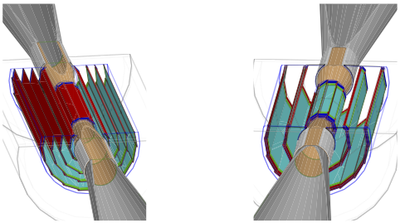
\includegraphics[width = 10 cm]{Pictures/vxd/ild_VXD.png}
     \caption{Overview of the two vertex detector option for the ILC. On the left, it is made of five single sided layers, whereas the right one represents three double-sided layers.}
   \end{figure}
   
   %They are two different geometrical designs under studied to build the \gls{VXD}. 
   %The first idea is to have a \gls{VXD} with five single-sided layers with a radii range from 15 to 60 mm.
   %The other option is to have three double-sided layers, which will have pixel sensors on both side separated by a mechanical structure of 2 mm thickness. 
   %The radii range is from 16 to 60 mm.

   Both geometry designs are embedding pixel sensors instead of strips or any other silicon devices.
   The different detector technologies under competition are:
    
   \subsubsection{FPCCD}
   
     The \gls{FPCCD} is based on the \gls{CCD} processes.
     It has a small pitch {$\simeq 5 \mu\text{m}$} which gives a sub-micron spatial resolution and an excellent capability to separate two near tracks.
     In order to limit the charge spread, the $15 \mu\text{m}$ epitaxial layer (the sensitive volume) is completely depleted.

   \subsubsection{DEPFET}
    
    The \gls{DEPFET} is an \gls{APS} in which field effect transistors are incorporated into each pixel.
    The sensor is completed depleted of free charged carries thanks to a voltage applied over the thickness.

    Rapid and efficient collection of signal on a deep implant underneath the field effect transistor
    Inside pixel: first amplification of signal
    Columns readout by two auxiliary \glspl{ASIC} while rows read out in rolling shutter mode.

   \subsubsection{CMOS}

   A third option is the integration of \gls{CMOS} pixel sensors. 
   The STAR experiment at RHIC is the first one to get an entire vertex detector made of ULTIMATE-MIMOSA28 CMOS sensors.
   One of the technology developed is described in section~\ref{sec:CMOS}.

  \section{PLUME}

  The \gls{PLUME} project aims to produce double-sided ladder prototypes with respect to the \gls{ILC} requirements.
  The collaboration is involving three labs in the Europe: the IPCH-PICSEL of Strasbourg, the University of Bristol and the DESY in Hamburg.
  All together, the collaboration is studying the feasibility to build such vertex detector using \gls{MAPS} thinned down to $50 \mu\text{m}$ and is exploring the benefits of this design.
  Strasbourg is in charge to develop and mount the sensors on the modules, to take care of the readout and the \gls{DAQ}, the cooling system.
  The mechanical design, stability measurements and building the ladders are done by the University of Bristol, while DESY studies the ladder mock-up, performs some power pulsing tests and is testing the modules in lab.
  The test beam was mainly done by Strasbourg until I've started yeah!

    \subsection{Design and goals}

    The figure~\ref{fig:PLUME} illustrates the design of a PLUME ladder.
    The mechanical structure is made of a 2 mm thick silicon-carbide foam which have a density varying between 8\% for the prototype build before 2011 and 4\% for the new ones.
    The choice of this foam is a good compromise between the stiffness and the thickness compare to other materials. \todo{REF Joel paper}
    It is macroscopically uniform and has the advantage to be easily machinable.
    Nevertheless, it has a low thermal conductivity (50 W/m/K) and can't be used to dissipate the heat.
    On each side, a low mass flex-cable is glued to power and to manage sensors from outside, via a connector on one edge.
    It is made of copper traces (prototype before 2011) or aluminum traces (new prototypes) coated in Kapton. 
    The ladder embeds twelve sensors, six on each face, that are glued and connected to the flex cable.
    At the moment, the design is dedicated to the MIMOSA-26 sensors thinned down to $50 \mu\text{m}$ but it could evolve to any kind of \gls{MAPS} sensors having the same thickness. 
    Although the MIMOSA-26 has a spatial resolution better than 3 $\mu$m, the integration time is not suited for the bunch train structures of the \gls{ILC}.

    The aims of the collaboration are to build ladders with a material budget better than 0.35 \% of $X_0$ for a spatial resolution better than 3 $\mu$m.

    \begin{figure}[!h]
      \centering
      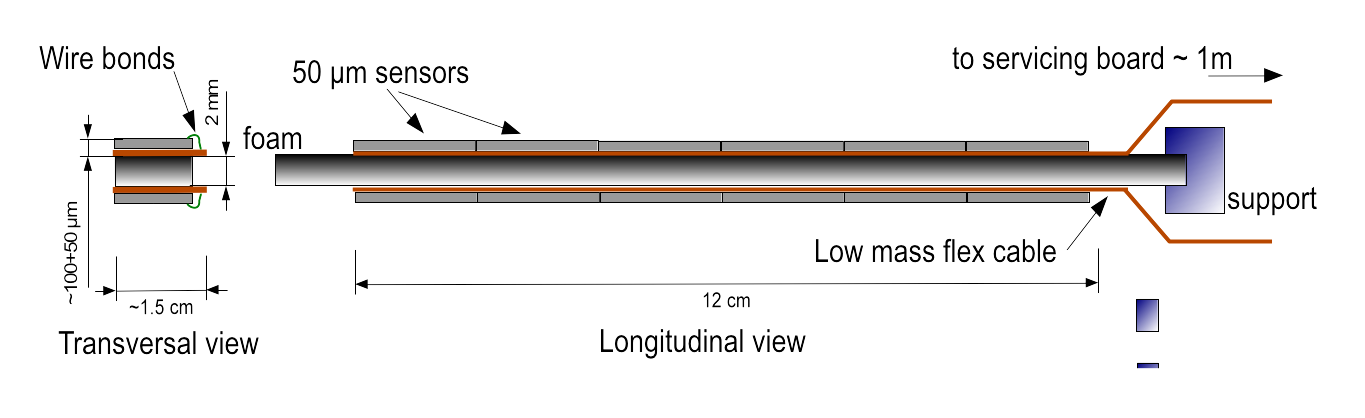
\includegraphics[width = 15 cm]{Pictures/vxd/plume_finalGoal.png}
      \caption{Side view (transversal and longitudinal) of the PLUME mechanical structure.}
      \label{fig:PLUME}
    \end{figure}

    \subsection{Prototypes}

    Before to reach the lightest ladder with a material budget of only 0.35 \%, the collaboration has studied the design, production and impact of the mechanical structure, but also how to power and control the sensors.
    
    The first ladder prototype (here labelled V0) was developed and test in 2009.
    It has two MIMOSA-20 analog output sensors on each side of a stiffener, providing a $1 \times 4 \text{ cm}^2$ sensitive area.
    As the purpose of this prototype was to settle the fabrication and the beam test procedure, the sensors and the flex-cables were not optimised.
     
    The second prototype featuring the final device design (V1) was developed in 2010. 
    The material budget is estimated to be 0.65 \% of $X_0$ in the sensor's sensitive area. 
    It is the first version to embed six MIMOSA-26 binary output sensors on each side of the stiffener that were working simultaneously.
    Two ladders were tested, one with 120 GeV pions at CERN-SPS in 2011 and the second one with positrons up to 5 GeV at DESY.
    The test beam at DESY is presented in chapter ... and some results of sensor's deformation observed at CERN are discussed in chapter ...

    The third prototype was mounted at the beginning of 2016 and has not been yet tested. 
    The traces thickness was reduced, the flex-cable width was adjust to the sensors width and the stiffener was made of a lower density Silicon Carbide foam reducing the material budget and the dead areas.

    \begin{table}
      \begin{center}
        \begin{tabular}{c c c c c c c}
        \hline %----------------------------
        \multirow{2}*{Layer}  & \multicolumn{3}{ c }{budget (\% X$_0$)}  \tabularnewline
                              &  V0 & V1 & Goal \tabularnewline
        \hline %----------------------------
        \hline %----------------------------
        Sensor                & 0.053 & 0.053 & 0.053 \tabularnewline
        Flex-cable            & 0.524 & 0.150 & 0.034 \tabularnewline
        Passive components    & 0     & 0.033 & 0.033 \tabularnewline
        Stiffener (foam)      & 0.764 & 0.175 & 0.087 \tabularnewline
        \hline %----------------------------
        \textbf{Total}        & 1.926 & 0.654 & 0.334 \tabularnewline
        \hline %----------------------------
        \end{tabular}
        \label{tab:X0}
        \caption{Estimation of the material budget for the different prototypes of the PLUME ladder.}
      \end{center}
    \end{table}

    \subsection{Perspectives}

    Although the collaboration has shown their expertise to build light mechanical structures, more tests and optimisations have to be done.
    MIMOSA-26 sensors are not designed to match the \gls{ILC} specs. 
    The integration time of this sensor is 115.2 $\mu$s, whereas the bunch train last only 0.95 ms (bunch crossing spaced out by 337 ns), a new CPS with a faster integration time has to be built.
    Although some tests were performed to used the power pulsing on the Mi-26 in order to decrease the power consumption, this sensors can't be used for that purpose\todo{Reference to paper from Oleg}.  

    The collaboration has to perform power pulsing test in a strong magnetic field to study the impact of the Laplace forces on the ladder and also the impact of the power pulsing on the capacity of the sensors.

  
  \section{Integration of CMOS sensors}
  \label{sec:CMOS}

  %Since the beginning of the 1990's, a new alternative to the \gls{CCD} was developed by the imaging industry: the \gls{APS}.
  %They are produced thanks to the \gls{CMOS} industrial process and are equipping nowadays the sensors of camera.
  %They are called so because the pixel is made of a photodiode associated to an active amplifier.
  %They are called active pixel sensors because the pixel is made of a photodiode  and an active amplifier. 
  %This technology is well used in the industry and equipped most of the camera produced.

  The PICSEL group of the IPHC of Strasbourg is developing since 1999 CMOS sensors called MIMOSA for \textit{Minimum Ionizing MOS Active pixel sensor}. 
  They are semi-conducting pixel sensors based on the \gls{APS}, an alternative to the \gls{CCD} developed at the beginning of the 1990's by the imaging industry and used nowadays for the smartphone's cameras.
  One particularity of the sensors developed by Strasbourg is that the different region of the sensor, such the sensitive area or the electronic layer where the signal is processed, are made of the same material.
  Such device is called then \gls{MAPS} and the different layers are:
  \begin{itemize}
    \item A substrate used as a bulk;
    \item An epitaxial layer which is the sensitive volume of the sensor;
    \item An electronic layer where are located the diodes collection charges and the micro-electronic that is processing the signal.
  \end{itemize}

  The motivation to use this technology or any other silicon sensor in particle physics is due to the minimum energy needed to create a electron/hole pair by a traversing particle.
  In silicon, this minimum energy is only 3.6 eV, while for a gaseous detector, it is close to 30 eV.
  %The first sensor developed by the PICSEL group of the IPHC of Strasbourg was born in 1999.
  %It was the first sensors prototype for physics of the PICSEL-family, called MIMOSA for \textit{Minimum Ionizing MOS Active pixel sensor}.
  %They are \gls{MAPS} because the sensitive

  %The PICSEL group of the IPHC of Strasbourg is developing \gls{MAPS} for the particle physics community since 1999.
  %They are called monolithic because the sensitive volume and the micro-electronic circuitry form one physical block.
  
    \subsection{Principle of a CMOS sensor}

    When a particle is traveling through matter, it loses energy via interaction with electrons and nuclei.
    For a thin layer of material, particles can cross all of the environment and lose a small fraction of their energy.
    It is admit that \gls{MIP} creates 80 e- per microns. 
    For thin layer energy lose describe by a Landau while thick material Gaussian.

%    \subsection{Architecture}
    \subsection{Charges creation and signal collection}   

    At the beginning, the micro-electronic industry was insulated the transistors from the substrate thanks to a high resistivity layer, called the epitaxial layer.
    The development of \gls{CMOS} sensors was done thanks to the properties offered by these semi-conductors.

    The different structure of the sensor has different doping.
    The bulk is a P++ doped layer made with a moderate quality silicon.
    The crystal structure has high defect crystal structure leading to a high rate recombination of charge carriers.
    Above the substrate, the epitaxial layer is P doped and made of a good quality silicon.
    The electron/hole pairs created in this layer don not recombine instantaneously like in a highly doped layer but they are thermally drifting. 
    
    The \gls{CMOS} sensors developed by the IPHC of Strasbourg are called monolithic \gls{MAPS} sensors because the different layers of the sensor are made in one block of the same material.
    The structure of the sensor is highly doped P+ substrate made of a moderate quality silicon. 
    It means that their are a lot of defaults in the crystal structure.
    This implies a high recombination rate of charge carriers.
    Above the bulk a layer made of good quality silicon to avoid the recombination of the charge carriers is grown.
    It is low doped P- and is called epitaxial layer. 
    It is the sensitive part of the sensor. 
    On top of the epitaxial layer, a N-wells implant has the role of the charge collection.
    The junction between the N-wells and the epitaxial layer create a P-N junction.
    At this junction, a depleted area is created that attracts the charge carriers.
    Nevertheless, this P-N junction is only one part of the pixel.
    Next to the N-wells implants are sitting highly doped P-well that reflect the charge carriers to the N-wells implants. 
    The difference of doping between the bulk and the epitaxial layer is also used to reflect charge carriers to the collection implants.

    The typical doping concentration are $10^{15} \text{at/cm}^3$ for the epitaxial layer, $10^{19} \text{at/cm}^3$ in the substrate and $10^{17} \text{at/cm}^3$ for the other layers.
    The doping concentration defines the size of the depleted region.

    As no external voltage is applied on the sensor to increase the depleted region, the charge carriers by particles are thermally diffused inside the sensitive volume to the diode.
    Nevertheless, the different doping concentration produces a built-in voltage defined as: 

    \begin{equation}
      V_b = \frac{kT}{q}ln\left( \frac{N_{p+}}{N_{p-}}\right)
    \end{equation}
    
    The build-in voltage depends on the Boltzmann constant $k$, the temperature $T$, the elementary charge $q$ and the different concentrations doping $N_{p\pm}$ of the interface.
    The charge collection efficiency is different from a fully-depleted sensor. 
    Indeed, the thermal diffusion 

    Charge carriers thermally diffused, their average path in epitaxial layer is longer than the on they would have in fully-depleted sensor.
    It is more likely that charge carriers are recombining in a non depleted sensor. 
    The charge collection efficiency is 

    \begin{figure}[!h]
      \centering
      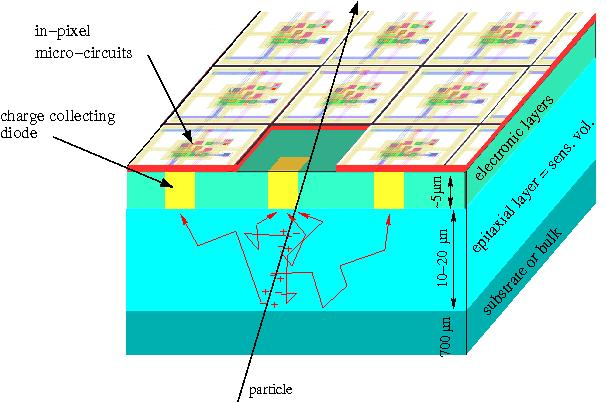
\includegraphics[width = 10cm]{Pictures/vxd/principeMapsMIP.jpg}
      \label{fig:principleMaps}
      \caption{Drawing of MAPS structure representing the different layers of the sensor and the path of charge carriers in the epitaxial layer.}
    \end{figure}

    The \gls{CMOS} sensors have several interesting properties.
    As this technology uses industrial process, the cost of fabrication is lower than other pixel technologies not based on an industrial process. 
    It allows to build many prototypes and build big matrix sensor.
    It also benefits from the industrial experience. 
    The CMOS technology are using smaller and smaller grid size (or more granular matrix).
    A pitch size of ten microns can be achieved. 
    As it was discussed before, due to the property of the small depleted area, the charge carriers tend to spread more over pixels.
    On the one hand, the signal is smaller per pixel, but the spatial resolution reconstructed with a centre of gravity algorithm is increasing.
    For example, binary output sensors with a pitch of 18.4 $\mu\text{m}$ can achieve a spatial resolution better than 3 $\mu\text{m}$.

    An other interesting property is coming from the doping of the different layers. 
    The bulk is not entirely responsible of the charge carriers reflection, only the interface between the substrate and the epitaxial layer is mainly responsible of the reflection.
    The substrate can be thinned down to few microns leading to a sensor with a thickness of 50 $\mu\text{m}$ while keeping the possibility to manipulate them.
    The material budget can then be reduced to 0.053 \%.

    As the epitaxial layer is thin, the signal collected by the diodes is small.
    A \gls{MIP} is creating 80 electron/hole pairs per microns, so the pixels are collecting between 1000 to more electrons.

    CMOS sensors are sensitive to ionizing and non-ionizing radiations that degrades the sensor properties.
    The non-ionizing radiation are damaging the crystal structure of the epitaxial layers, creating default in the lattice.
    The recombination rate is increasing and reduces the signal collected.
    To avoid this effect, two solutions are possible.
    The first one is to reduce the size of the pixels to decrease the path of the particles from the epitaxial layer to collection diodes.
    Nevertheless, the cost to build sensors with a smaller pitch is increasing.
    The second solution is to increase the resistivity of the epitaxial layer to increase the depleted area.
    
    The ionizing radiation are responsible of charges accumulation in the electronic layer.
    The leakage current is increasing in the pixel and diode collection.
    To reduce the leakage current, smaller diodes can be used to reduce the impact of the leakage current but as it was explained before, the cost of fabrication is increasing.
    
    \subsection{Signal processing}

    If no charge is collected by the pixel, the voltage at the equivalent capacitor of the diode is evolving because of the leakage current inherent in the junction.
    The pixel reading can be done in two different ways, depending on the method used to minimise the leakage current effect.
    Currently, two pixel architectures are used to compensate the diode's leakage current: the \textit{3 Transistors pixel design}, mainly used in imaging, and the \textit{self-biased pixel design}.
    The circuit diagram shown on the figure~\ref{fig:elecArch} represents the two pixel design methods.
    The first one, corresponding to the left part of the circuit diagram, consists to reinitialise the collection diode's voltage to a reference voltage thanks to a \textit{reset} transistor, denoted M1 on the diagram.
    This method works in two steps. 
    Firstly, the M1 transistor is closed and the charge of the equivalent capacitor $C_d$ associated to the junction P-N, represented by a diode on the diagram, is slowly decreasing because of the diode's leakage current. 
    During this phase, the pixel is sensitive and is read.
    After a time interval equivalent to the integration time of the sensor, the transistor M1 is opened to recharge $C_d$ to its initial voltage.
    During this time, the pixel is not sensitive.
    While M1 is used for the reset, M2 is used as a pre-amplifier of the signal created by the diode and M3 link up the voltage to the output of the circuit.
    Although this compensation method is fast, it generates a dead time for detection between two readings.
    
   % The first method consists to force time to time the reinitialisation of the voltage on the collection diode leads to a reference value thanks to a \textit{reset} transistor.
   % In order to limit the impact of the noise created by thermal fluctuations during the reinitialisation, a \textit{correlated double sampling} is used. A first voltage reading from output of the pixel stores the \textit{reset} level and a second reading subtracts the measured voltage previously read to reduce the noise impact.
   % Although the compensation is fast, it generates a dead time for detection between two readings.
    
    The \textit{self-biased pixel design} method using a p-n junction, symbolised by a diode mounted in the other direction, in the n-well coupled to the collection diode but mounted in the other way to absorb the leakage current.
    Using a forward p-n junction has the advantage to avoid any dead-time because the diode's leakage current is continuously compensated by the second diode.
    While no particle is crossing the sensor, there is an equilibrium between the leakage and recharge current.
    When a particle is crossing the sensor, the charges are collected by the pixel, leading to a discharge of the diode's capacitor $C_d$, which is followed by a recharge to reach again the equilibrium.
    Nevertheless, the recharge procedure should be slower than the integration time to be able to detect physics signal during detection.
    Indeed, when the recharge is too fast, the physics signal is masked the passage of particle will never be notified.
    Even if the time interval to recharge the capacitor $C_d$ is set properly, an important charge collection per pixel could disturb the recharge phase and the pixel will reach a stable level again only a long time interval of the order of 10 ms.

    \begin{figure}[!h]
      \missingfigure{Electric sketch}
      \label{fig:elecArch}
      \caption{Two different architectures of pixel. The left one is a pixel of type 3T, whereas the right one is a self-biased one.}
    \end{figure}

    TALK ABOUT READOUT

    \begin{figure}[!h]
      \missingfigure{Rolling shutter}
      \label{fig:rollShut}
      \caption{Parallel column readout.}
    \end{figure}

    TALK ABOUT NOISE

    \gls{FPN} and \gls{TN}
    \begin{itemize}
      \item[Noise during reset]
      \item[Noise during integration]
      \item[Noise during readout]
    \end{itemize}

    The chapter~\ref{chap:labTests} describes the steps to characterise the fixed pattern noise and temporal noise.


    \subsection{State of the art in high energy physics}

    The PICSEL group has developed sensors, called or ULTIMATE, for the STAR experiment at Brookhaven National Laboratory\todo{REF to a paper}.
    They are based on \gls{MIMOSA}-28 sensors and are integrated into the vertex detector.
    The figure~\ref{fig:Mi28} is showing a half-section of the STAR vertex detector (subfigure~\ref{fig:vxdSTAR}) and a \gls{MIMOSA}-28 bounded on a PCB.
    The choice for this technology was made because of their characteristics.
    Indeed, the thickness of a sensor is around 50 $\mu\text{m}$ in order to minimise the multiple scattering of particles.
    The matrix is made of roughly $9 \times 10^5$ pixels, corresponding to 960 columns and 928 rows for a pitch of 20.7 x 20.7 $\mu\text{m}^2$.
    The sensitive area is 19.7 x 19.2 $\text{cm}^2$.
    They have a binary output integrating a zero suppression technology (SUZE) and the integration time of the whole matrix is 200 $\mu\text{s}$.
    Thanks to this architecture, the sensors can reach a particle detection rate of $10^6$ particles/$\text{cm}^2$/s. 
    Finally, their power consumption is lower or equal to 150 mW/$\text{cm}^2$.
    The spatial resolution obtained for ULTIMATE is less than 4 $\mu\text{m}$.

  \begin{figure}[!h]
    \centering
    \begin{subfigure}[t]{0.3\textwidth}
        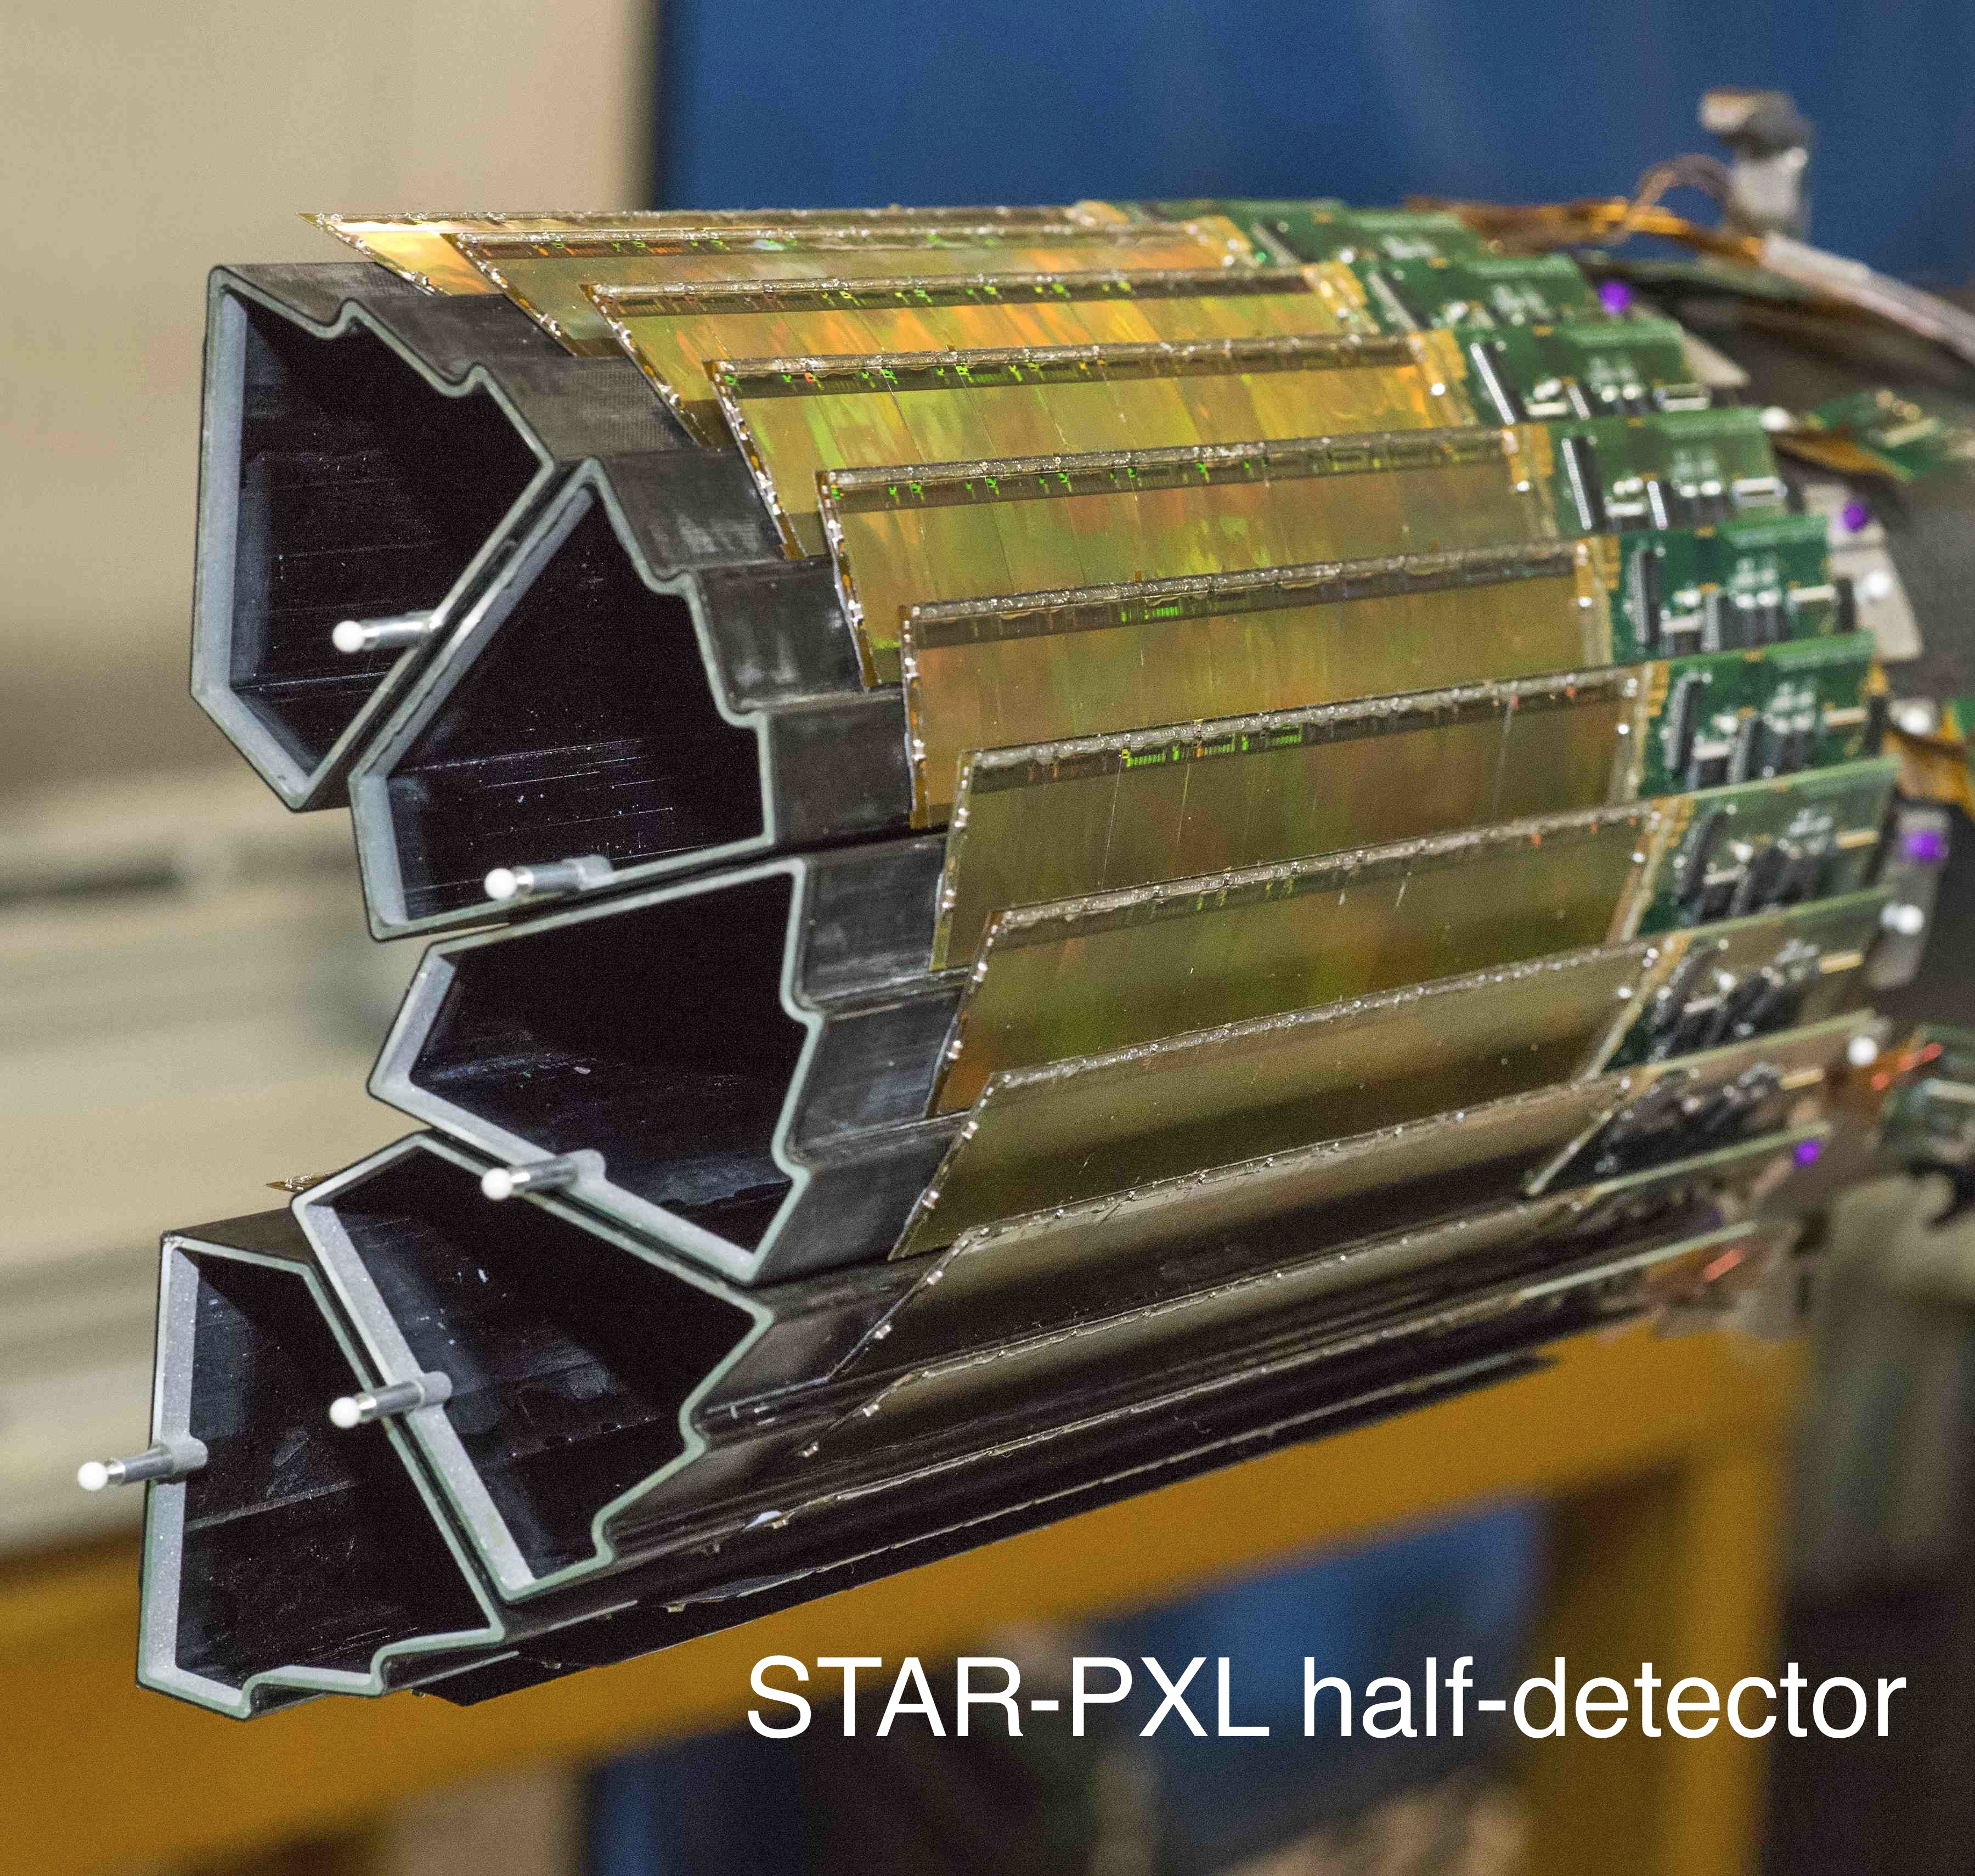
\includegraphics[width=\textwidth]{Pictures/vxd/pxlFinal_sideView_smallSize.jpg}
        \caption{Half part picture of the pixel vertex detector at STAR.}
        \label{fig:vxdSTAR}
    \end{subfigure}
    \qquad
     %add desired spacing between images, e. g. ~, \quad, \qquad, \hfill etc. 
      %(or a blank line to force the subfigure onto a new line)
    \begin{subfigure}[t]{0.3\textwidth}
        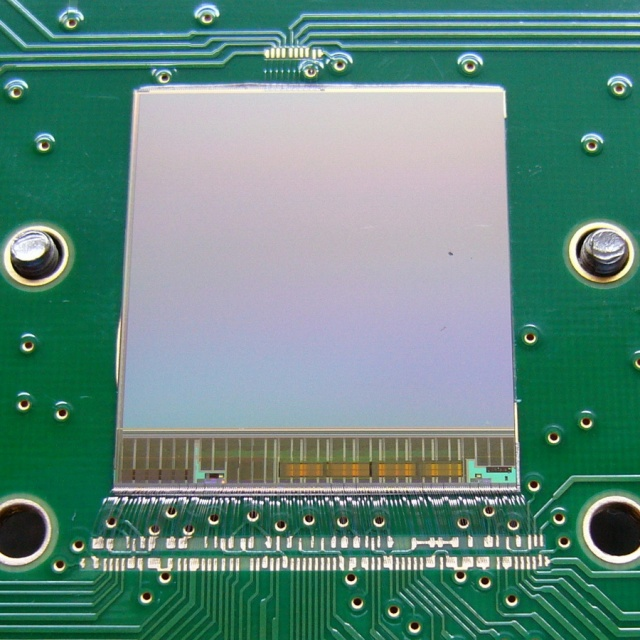
\includegraphics[width=0.95\textwidth]{Pictures/vxd/ultimate2.jpg}
        \caption{ULTIMATE chip bounded on a PCB. The top wire bounds are used for a slow analog output dedicated to lab test, while the bottom ones are the wire bounds which control and read the sensor. }
        \label{fig:ultimate}
    \end{subfigure}
    \caption{Pictures of the STAR vertex detector and an ULTIMATE chip}\label{fig:Mi28}
    \end{figure}    

An older version of the \gls{MIMOSA}-28, based on the same architecture is currently used on the \gls{PLUME} ladder: \gls{MIMOSA}-26.
    Contrary to his brother, the matrix contains roughly $7 \times 10^5$ pixels, distribute on 1152 columns and 576 rows.
    The pixels are scared with a pitch of 18.4 $\mu\text{m}$ and the sensitive area is 21.2 x 10.6 $\text{cm}^2$.
    They also have a binary output integrating a zero suppression mode but the integration time of the whole matrix is 115.2 $\mu\text{s}$.
    The architecture of a \gls{MIMOSA}-26 is represented on figure~\ref{fig:archMi26}
    This sensors are equipping the telescope planes at DESY and CERN.

    \begin{figure}[!h]
      \missingfigure{Architecture of Mi26}
      \label{fig:archMi26}
      \caption{Layout of the MIMOSA-26 matrix.}
    \end{figure}
    


